\chapter{\IFRU{Указатели}{Pointers}}
\index{\CLanguageElements!\Pointers}
\label{label_pointers}

\newcommand{\ttf}{\TT{f1()}}

\IFRU{Указатели также часто используются для возврата значений из функции (вспомните случай
со \scanf{}~(\ref{label_scanf}))}
{Pointers are often used to return values from function (recall \scanf case~(\ref{label_scanf}))}.
\IFRU{Например, когда функции нужно вернуть сразу два значения}
{For example, when function should return two values}.

\section{\IFRU{Пример с глобальными переменными}{Global variables example}}

\lstinputlisting{patterns/061_pointers/global.c}

\IFRU{Это компилируется в}{This compiling into}:

\lstinputlisting[caption=\Optimizing MSVC 2010 (/Ox /Ob0)]{patterns/061_pointers/global.asm}

\index{\olly}
\IFRU{Посмотрим это в}{Let's see this in} \olly: \figname \ref{fig:pointers_olly_global_1}.
\IFRU{В начале адреса обоих глобальных переменных передаются в}{At first, global
variables addresses are passed into} \ttf.
\IFRU{Можно нажать}{We can click} ``Follow in dump'' \IFRU{на элементе стека и в окне слева 
увидим место в сегменте данных выделенных для двух переменных}{on the stack element, and we will see 
a place in data segment allocated for two variables}.
\IFRU{Эти переменные обнулены, потому что, по стандарту, неинициализированные данные (\ac{BSS}) 
обнуляются перед началом исполнения}
{These variables are cleared, because non-initialized data (\ac{BSS}) are cleared before
execution begin}.
\IFRU{И они находятся в сегменте данных, о чем можно удостовериться нажав}
{They are residing in data segment, we can be sure it is so, by pressing} Alt-M \IFRU{и увидев карту
памяти}{and seeing memory map}: \figname \ref{fig:pointers_olly_global_5}.

\IFRU{Трассируем}{Let's trace} (F7) \IFRU{до начала исполнения}{until execution of} \ttf 
\figname \ref{fig:pointers_olly_global_2}.
\IFRU{В стеке видны и значения}{Two values are seen in the stack} $456$ (\TT{0x1C8}) \AndENRU 
$123$ (\TT{0x7B}), \IFRU{а также адреса двух глобальных переменных}{and two global variables addresses
as well}.

\IFRU{Трассируем до конца}{Let's trace until the end of} \ttf.
\IFRU{Мы видим в окне слева, как результаты вычисления появились в глобальных переменных}
{At the window at left we see how calculation results are appeared in the gloval variables} 
\figname \ref{fig:pointers_olly_global_3}.

\IFRU{Теперь из глобальных переменных значения загружаются в регистры для передачи в}
{Now values of global variables are loaded into registers for passing into} \printf:
\figname \ref{fig:pointers_olly_global_4}.

\begin{figure}[H]
\centering
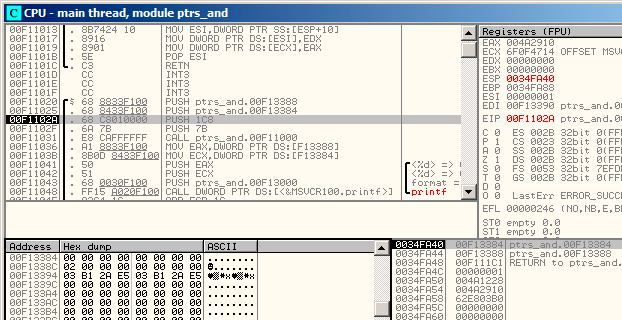
\includegraphics[scale=0.66]{patterns/061_pointers/olly_global1.png}
\caption{\olly: \IFRU{передаются адреса двух глобальных переменных в}
{global variables addresses are passing into} \ttf}
\label{fig:pointers_olly_global_1}
\end{figure}

\begin{figure}[H]
\centering
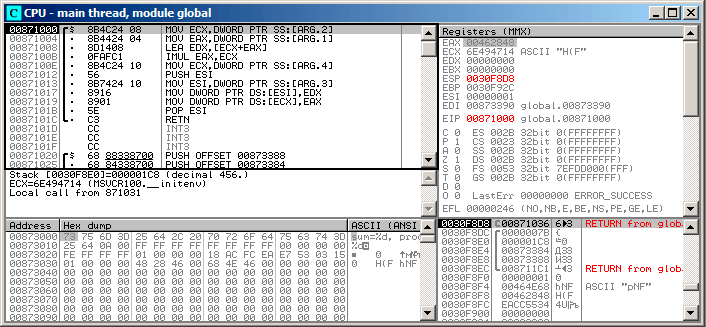
\includegraphics[scale=0.66]{patterns/061_pointers/olly_global2.png}
\caption{\olly: \IFRU{начало работы \ttf}{\ttf is started}}
\label{fig:pointers_olly_global_2}
\end{figure}

\begin{figure}[H]
\centering
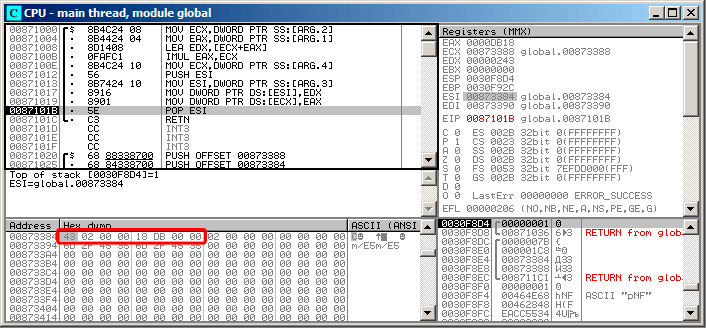
\includegraphics[scale=0.66]{patterns/061_pointers/olly_global3.png}
\caption{\olly: \ttf \IFRU{заканчивает работу}{finishes}}
\label{fig:pointers_olly_global_3}
\end{figure}

\begin{figure}[H]
\centering
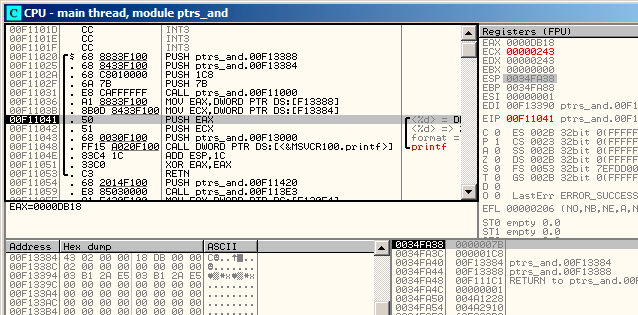
\includegraphics[scale=0.66]{patterns/061_pointers/olly_global4.png}
\caption{\olly: \IFRU{адреса глобальных переменных передаются в}
{global variables addresses are passed into} \printf}
\label{fig:pointers_olly_global_4}
\end{figure}

\begin{figure}[H]
\centering
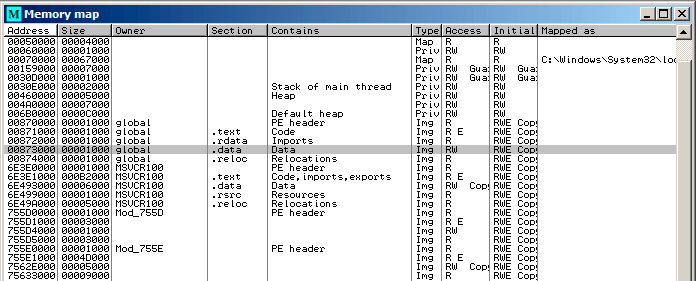
\includegraphics[scale=0.66]{patterns/061_pointers/olly_global5.png}
\caption{\olly: \IFRU{карта памяти}{memory map}}
\label{fig:pointers_olly_global_5}
\end{figure}

\section{\IFRU{Пример с локальными переменными}{Local variables example}}

\IFRU{Немного переделаем пример}{Let's rework our example slightly}:

\lstinputlisting[caption=\IFRU{теперь переменные локальные}
{now variables are local}]{patterns/061_pointers/local_\LANG.c}

\RU{Код ф-ции }\ttf \IFRU{не изменится}{function code will not changed}.
\IFRU{Изменится только \main}{Only \main code will}:

\lstinputlisting[caption=\Optimizing MSVC 2010 (/Ox /Ob0)]{patterns/061_pointers/local.asm}

\newcommand{\PtrsAddresses}{\TT{0x35FCF4} \AndENRU \TT{0x35FCF8}\xspace}

\IFRU{Снова посмотрим в}{Let's again take a look into} \olly.
\IFRU{Адреса локальных переменных в стеке это}{Local variable addresses in the stack are} \PtrsAddresses.
\IFRU{Видно как они заталкиваются в стек}{We see how these are pushed into the stack}: 
\figname \ref{fig:pointers_olly_stk_1}.

\IFRU{Начало работы \ttf}{\ttf is started}.
\IFRU{В стеке по адресам}{Random garbage are at} \PtrsAddresses \IFRU{пока находится случайный мусор}
{so far} \figname \ref{fig:pointers_olly_stk_2}.

\IFRU{Конец работы \ttf}{\ttf finished}.
\IFRU{В стеке по адресам \PtrsAddresses теперь значения \TT{0xDB18} \AndENRU \TT{0x243}, 
это результаты работы \ttf}
{There are \TT{0xDB18} \AndENRU \TT{0x243} now at \PtrsAddresses addresses, these values are
\ttf function result}.

\begin{figure}[H]
\centering
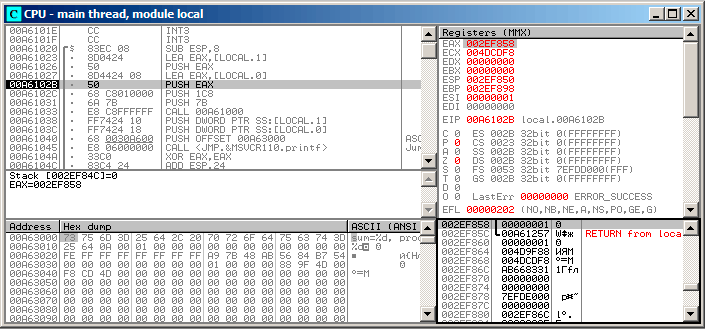
\includegraphics[scale=0.66]{patterns/061_pointers/olly_stk1.png}
\caption{\olly: \IFRU{адреса локальных переменных заталкиваются в стек}{addresses of local variables are
pushed into the stack}}
\label{fig:pointers_olly_stk_1}
\end{figure}

\begin{figure}[H]
\centering
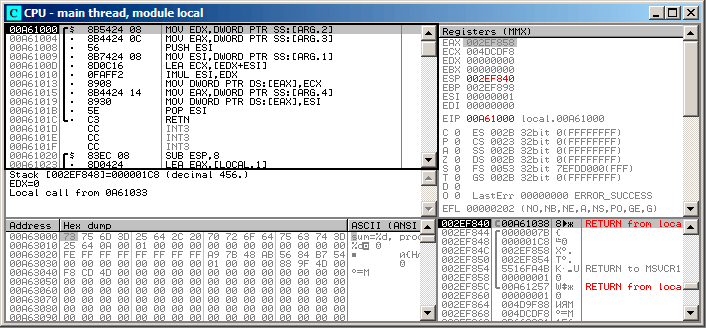
\includegraphics[scale=0.66]{patterns/061_pointers/olly_stk2.png}
\caption{\olly: \ttf \IFRU{начинает работу}{starting}}
\label{fig:pointers_olly_stk_2}
\end{figure}

\begin{figure}[H]
\centering
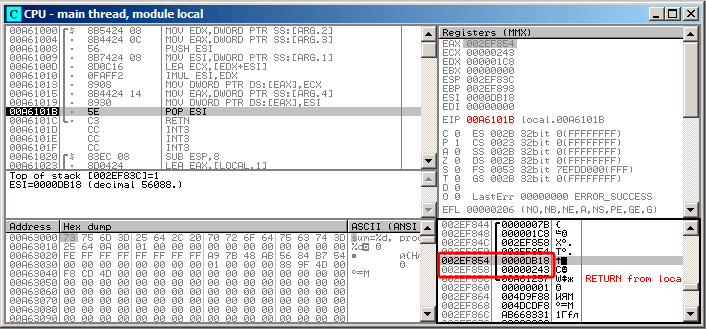
\includegraphics[scale=0.66]{patterns/061_pointers/olly_stk3.png}
\caption{\olly: \ttf \IFRU{заканчивает работу}{finished}}
\label{fig:pointers_olly_stk_3}
\end{figure}

\section{\IFRU{Вывод}{Conclusion}}

\IFRU{\ttf может одинаково хорошо возвращать результаты работы в любые места памяти, 
находящиеся где угодно}{\ttf can return results to any place in memory, located anywhere}.
\IFRU{В этом суть и удобство указателей}{This is essence and usefulness of pointers}.

\IFRU{Кстати,}{By the way, \Cpp} \IT{references} \IFRU{в \Cpp работают точно так же}{works just in the
same way}. \IFRU{Читайте больше об этом}{Read more about them}: (\ref{cpp_references}).

